\section{Theorie}
\label{sec:Theorie}

\noindent Geiger-Müller Zählrohre dienen zur Detektion radioaktiver Strahlung, welche in der Regel aus $\text{He-}4$ Atomkernen,
der $\alpha$-Strahlung, oder Elektronen, der $\beta^-$ Strahlung, besteht. Dabei nutzen die Rohre aus, dass diese 
Strahlung ionisierend wirkt. Je nach Energie, mit der die Strahlung eintrifft treten jedoch unterschiedliche Effekte auf.

\subsection{Detektion der Strahlung}

\noindent Nach außen hin ist ist das Zählrohr von einem Metallmantel umgeben und in der Mitte des Zylinders ist ein Metalldraht.
Zwischen dem Mantel und dem Draht ist eine Spannung angelegt, wobei die Wand als Kathode und der Draht als Anode
wirken soll. In dem Zylinder befindet sich zusätzlich ein Gas, welches durch die einfallende Strahlung ionisiert
werden kann. Die bei der Ionisierung entstanden Elektronen und Ionen, werden dann zu der entsprechenden Elektrode
beschleunigt. Beim Auftreffen kommt es dann zu einem großen Spannungsabfall, welcher dann gemessen wird.

\begin{figure}
    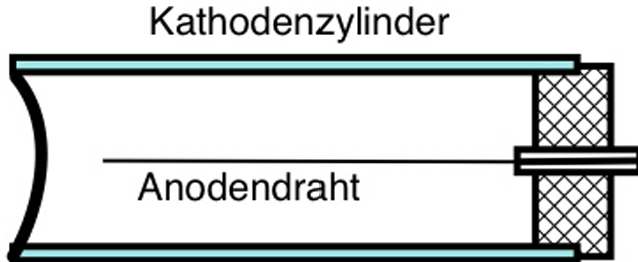
\includegraphics{Bilder/zaelrohr.png}
    \caption{Schematischer Aufbau des inneren eines Geiger-Müller Zählrohrs.}
    \label{fig:geiger}
\end{figure}

\subsection{Effekte auf die Elektronen im Gas}

\noindent Während die Elektronen beschleunigt werden, kollidieren diese mit dem Gas, welches in dem  Zylinder ist.
Wenn die Spannung im Zylinder zu niedrig ist, dann werden die Elektronen von den anderen Atomen wieder eingefangen.
in einem Prozess, der rekombination genannt wird. Für steigende Spannung wird dieser Effekt immer insignifikanter bis
ein Spannungsplateu erreicht wird. \\
\noindent Dieses Intensitätsplateusplateu befindet sich in einem Bereich, der Ionisationskammer genannt wird. In diesem Bereich
werden nur diejenigen Ladungen detektiert, die auch durch die Strahlung freigesetzt werden.\\
\noindent Der nächste Spannungsbereich ist dadurch gekennzeichnet, dass die lösgelösten Elektronen selbst genügend Energie
besitzen um selbst weitere Elektronen aus anderen Atomen mit der Stoßionisation loszulösen. Dieser Effekt wird in der 
Nähe des Anodendrahtes dann weiter verstärkt sodass die neu gelösten Elektronen zusätzlich andere Elektronen loslösen
können. Dadurch entsteht eine Kaskade aus geladenen Teilchen, die auch Townsend-Lawine genannt wird. Die Größenordnung
der zusätzlich detektierten Ladungen hängt dabei von der Energie der einfallenden Strahlung ab, wodurch es dann möglich
ist die Strahlungstypen voneinander zu unterscheiden.\\
\noindent Wenn die Spannung groß genung wird, dann können einzelne Atome genügend angeregt sein, sodass diese Photonen
emmitieren. Für diese ist es wiederum auch möglich Elektronen zu lösen und es kommt durch die hohe Spannung im ganzen
Zylinder zu Townsend-Lawinen. Dieser Effekt kann mit einem Löschgas, wie Alkohole unterdrückt werden, da dieses dann die
Photonen wieder absorbiert.  Da die Elektronen durch ihre geringe Trägheit deutlich schneller beschleunigt werden,
bleiben um die Anode die positiven Ionenrümpfe übrig, die weitere Elektronen daran hinderen zu passieren. Es würde dadurch 
zu einem weiteren Intensitätsplateu kommen. Allerdings entstehen bei dem Aufstoß der Ionen an der Kathode sekundäre
Elektronen, die zwar durch das Löschgas gedämpft werden können, aber zeitlich verzögerte Impulse auslösen können.
Die dadurch entstehende Steigung ist über die relative Zählrate
\begin{equation}
    s=\frac{\delta N}{N} \dot 100\frac{\unit{\percent}}{100\unit{\volt}}
    \label{eqn:relativ}
\end{equation}
bestimmt. Dieser Bereich wird Geiger-Müller Bereich genannt, da das Zählrohr für gewöhnlich in diesem Bereich betrieben wird.\\
\noindent Irgenwann ist die Spannung jedoch groß genung, dass diese selbst das Gas ionisiert und es somit wieder zu einem 
stetigen Anstieg kommt.

\begin{figure}[H]
    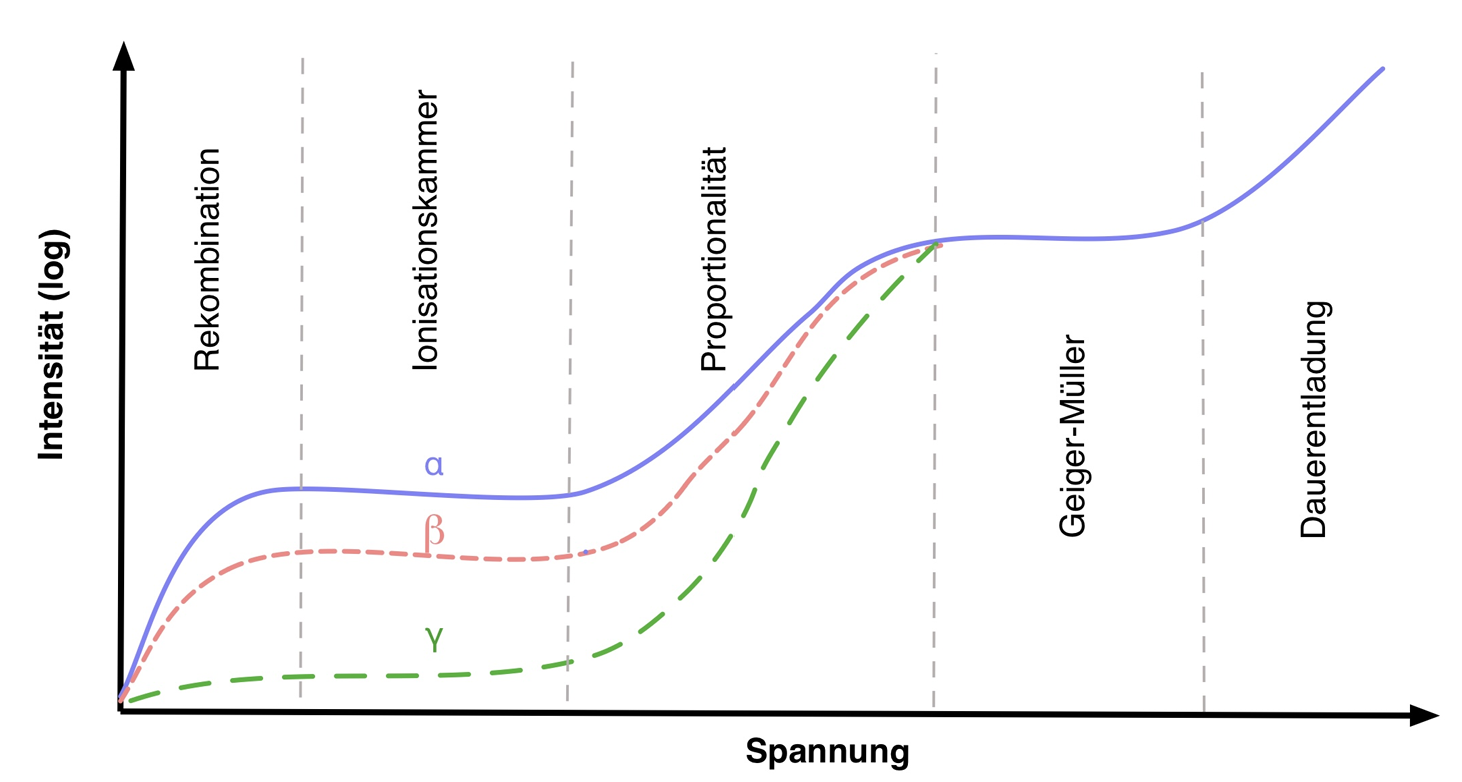
\includegraphics{Bilder/intensitaetsverlauf.png}
    \caption{Der gesamte oben beschriebene Verlauf der Intensität der detektierten Teilchen in Abhängigkeit zu der Spannung
    in dem Zählrohr}
    \label{fig:intens}
\end{figure}

\noindent Desweiteren entsteht im Zählrohr in dem Geiger-Müller Bereich eine sogenannte Totzeit $\tau$, in der keine
Strahlung detektiert werden kann. Dies liegt daran, dass die Ionenrümpfe um die Anode herum weitere Lawinen verhindern
und somit erst dispersieren, damit das Zählrohr wieder Impulse messen kann. Die Totzeit kann mit
\begin{equation}
    \tau=\frac{N_1+N_2-N_{12}}{2N_1N_2}
    \label{eqn:totzeit}
\end{equation}
bestimmt werden, wobei $N_1$ und $N_2$ die Anzahl der detektierten Pulse über einen bstimmten Zeitraum ist
und $N_{12}$ die gleiche Messung nur mit beiden Quellen zusammen.

\cite{V703}